\documentclass[tikz,border=4pt]{standalone}

\usepackage[T1]{fontenc}
\usepackage[utf8]{inputenc}
\usepackage{helvet}
\renewcommand{\familydefault}{\sfdefault}
\usepackage{tikz}
\usetikzlibrary{arrows.meta,fit,backgrounds,calc}

\definecolor{noirbg}{HTML}{131B24}
\definecolor{noirpanel}{HTML}{1C2834}
\definecolor{noirpanelalt}{HTML}{2A3948}
\definecolor{noirtext}{HTML}{ECF1F4}
\definecolor{noirmuted}{HTML}{C4CDD5}
\definecolor{duneorange}{HTML}{F2682B}
\definecolor{noircyan}{HTML}{92DDF2}
\definecolor{noirmint}{HTML}{96D6AE}

\tikzset{
  stage/.style={
    draw=noirmuted,
    rounded corners=4pt,
    semithick,
    minimum height=1.05cm,
    align=center,
    font=\sffamily\small,
    fill=noirpanel,
    text=noirtext,
    inner sep=5pt
  },
  hot/.style={stage, draw=duneorange, very thick, fill=noirpanelalt},
  future/.style={stage, draw=noirmint, very thick, fill=noirpanelalt},
  shared/.style={stage, draw=noircyan, semithick},
  reject/.style={
    rounded corners=10pt,
    semithick,
    minimum height=0.72cm,
    align=center,
    font=\sffamily\scriptsize,
    fill=noirpanel,
    text=noirtext,
    inner sep=4pt
  },
  callout/.style={
    rounded corners=4pt,
    semithick,
    fill=noirbg,
    align=center,
    font=\sffamily\scriptsize,
    text=noirmuted,
    inner sep=4pt
  },
  flow/.style={-{Latex[length=2.4mm]}, thick, draw=noirmuted},
  accent/.style={-{Latex[length=2.2mm]}, semithick, draw=duneorange},
  subtle/.style={-{Latex[length=2.0mm]}, semithick, dashed, draw=noircyan}
}


\begin{document}
\pagecolor{noirbg}
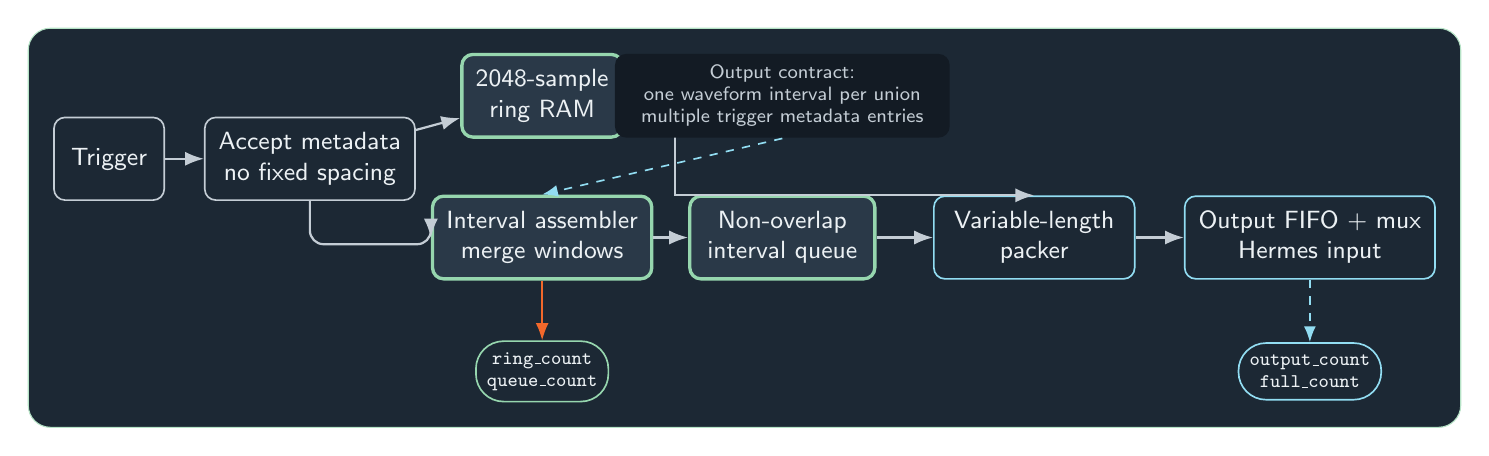
\begin{tikzpicture}[x=1cm,y=1cm]

\node[stage, minimum width=1.4cm] (arrival) at (0.0,0.75) {Trigger};
\node[stage, minimum width=2.5cm] (gate) at (2.55,0.75) {Accept metadata\\no fixed spacing};
\node[future, minimum width=2.0cm] (ring) at (5.5,1.55) {2048-sample\\ring RAM};
\node[future, minimum width=2.35cm] (assembler) at (5.5,-0.25) {Interval assembler\\merge windows};
\node[future, minimum width=2.35cm] (queue) at (8.55,-0.25) {Non-overlap\\interval queue};
\node[shared, minimum width=2.55cm] (packer) at (11.75,-0.25) {Variable-length\\packer};
\node[shared, minimum width=2.85cm] (out) at (15.25,-0.25) {Output FIFO + mux\\Hermes input};

\draw[flow] (arrival) -- (gate);
\draw[flow] (gate) -- (ring);
\draw[flow, rounded corners=5pt] (gate.south) -- ++(0,-0.55) -| (assembler.west);
\draw[flow] (ring.east) -- ++(0.65,0) |- (packer.north);
\draw[flow] (assembler) -- (queue);
\draw[flow] (queue) -- (packer);
\draw[flow] (packer) -- (out);

\node[reject, draw=noirmint] (local) at (5.5,-1.95) {\texttt{ring\_count}\\\texttt{queue\_count}};
\node[reject, draw=noircyan] (full) at (15.25,-1.95) {\texttt{output\_count}\\\texttt{full\_count}};
\draw[accent] (assembler.south) -- (local.north);
\draw[subtle] (out.south) -- (full.north);

\node[callout, minimum width=4.25cm] (contract) at (8.55,1.55)
  {Output contract:\\one waveform interval per union\\multiple trigger metadata entries};
\draw[subtle] (contract.south) -- (assembler.north);

\begin{pgfonlayer}{background}
  \node[
    draw=noirmint!70,
    rounded corners=8pt,
    fill=noirpanel,
    fit=(arrival)(out)(local)(full)(contract),
    inner sep=9pt
  ] {};
\end{pgfonlayer}

\end{tikzpicture}
\end{document}
